% Top 10 laws by definition count with defect rates
% Data from pipeline run on 5,799 definitions
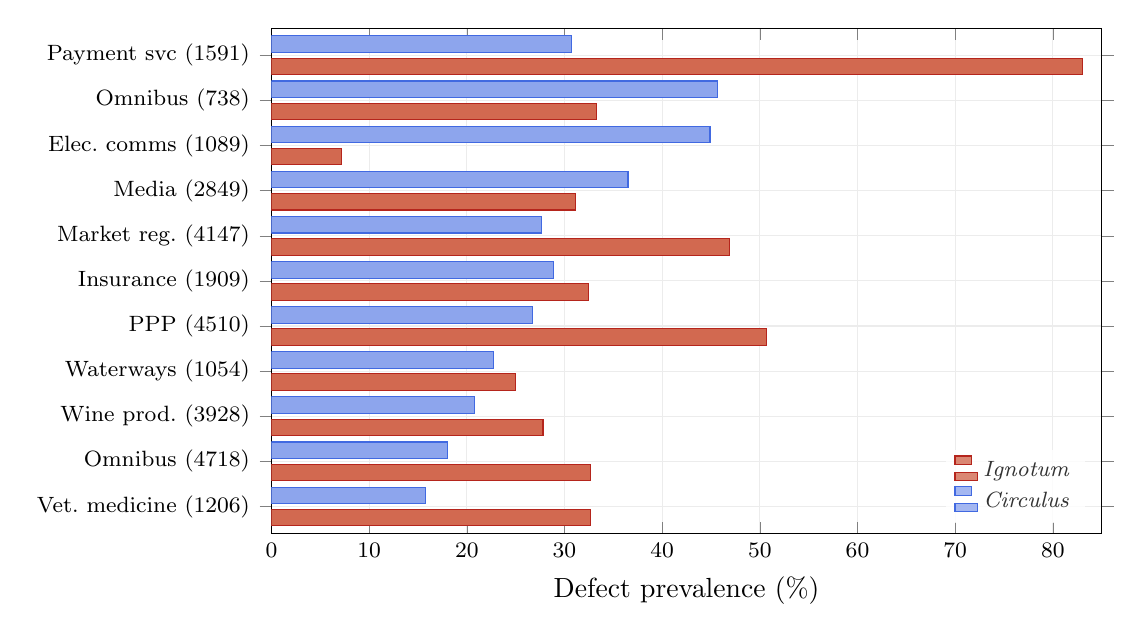
\begin{tikzpicture}
\begin{axis}[
  width=\linewidth,
  height=8cm,
  xbar,
  xlabel={Defect prevalence (\%)},
  xmin=0, xmax=85,
  ytick=data,
  yticklabels={
    {Vet.\ medicine (1206)},
    {Omnibus (4718)},
    {Wine prod.\ (3928)},
    {Waterways (1054)},
    {PPP (4510)},
    {Insurance (1909)},
    {Market reg.\ (4147)},
    {Media (2849)},
    {Elec.\ comms (1089)},
    {Omnibus (738)},
    {Payment svc (1591)}
  },
  yticklabel style={font=\footnotesize},
  xticklabel style={font=\footnotesize},
  legend style={at={(0.98,0.02)}, anchor=south east, font=\footnotesize, draw=none, fill=white, fill opacity=0.8},
  bar width=6pt,
  grid=major,
  grid style={gray!15},
  enlarge y limits=0.06,
]

% Ignotum per ignotum
\addplot[fill=BrickRed!60, draw=BrickRed] coordinates {
  (32.7,0) (32.7,1) (27.8,2) (25.0,3) (50.7,4) (32.5,5) (46.9,6) (31.1,7) (7.2,8) (33.3,9) (83.0,10)
};
\addlegendentry{\emph{Ignotum}}

% Circulus in definiendo
\addplot[fill=RoyalBlue!60, draw=RoyalBlue] coordinates {
  (15.8,0) (18.0,1) (20.8,2) (22.7,3) (26.7,4) (28.9,5) (27.6,6) (36.5,7) (44.9,8) (45.7,9) (30.7,10)
};
\addlegendentry{\emph{Circulus}}

\end{axis}
\end{tikzpicture}
